\documentclass[]{article}

\usepackage[sc]{mathpazo} % Use the Palatino font
\usepackage[T1]{fontenc} % Use 8-bit encoding that has 256 glyphs
\linespread{1.05} % Line spacing - Palatino needs more space between lines
\usepackage{microtype} % Slightly tweak font spacing for aesthetics

\usepackage[hmarginratio=1:1,top=32mm,columnsep=20pt]{geometry} % Document margins
\usepackage[hang, small,labelfont=bf,up,textfont=it,up]{caption} % Custom captions under/above floats in tables or figures
\usepackage{booktabs} % Horizontal rules in tables
\usepackage{float} % Required for tables and figures in the multi-column environment - they need to be placed in specific locations with the [H] (e.g. \begin{table}[H])
\usepackage{hyperref} % For hyperlinks in the PDF
\usepackage{graphicx} 

\usepackage{lettrine} % The lettrine is the first enlarged letter at the beginning of the text
\usepackage{paralist} % Used for the compactitem environment which makes bullet points with less space between them

\usepackage{titlesec} % Allows customization of titles
\renewcommand\thesection{\Roman{section}} % Roman numerals for the sections
\renewcommand\thesubsection{\Roman{subsection}} % Roman numerals for subsections
\titleformat{\section}[block]{\large\scshape\centering}{\thesection.}{1em}{} % Change the look of the section titles
\titleformat{\subsection}[block]{\large}{\thesubsection.}{1em}{} % Change the look of the section titles

\title{Using Gaussian Process for Multi-objective optimization}

\author{Daqing Yi
%\affil{Brigham Young University}
}
\date{}

\begin{document}

\maketitle

\section{Active learning for multi-objective optimization}

\begin{itemize}
\item [\textbf{2013}] Active learning for multi-objective optimization~\cite{zuluaga2013active}
\item [\textbf{2012}] "Smart" Design Space Sampling to Predict Pareto-optimal Solutions~\cite{Zuluaga2012} 
\end{itemize}

\emph{Pareto Active Learning} (PAL) is proposed to solve the multi-objective optimization problem, which samples design space to predict Pareto-optimal set.
The process includes
\begin{itemize}
\item modeling the objectives as samples from a Gaussian process distribution;
\item choosing next design;
\item controlling prediction accuracy and sampling cost.
\end{itemize}

\begin{tabular}{|c|c|} \hline
design space $ E \subset \mathbb{R}^{d} $ & objective space $ f(E) \subset \mathbb{R}^{n} $ \\ \hline
Pareto-optimal set $ P $ & Pareto front $ f(P) $ \\ \hline
\end{tabular}

$ P $ - positive, 
$ N $ - negative, 
$ U $ - unclassified, 
$ S $ - evaluated set and $ R $ - uncertainty region.

The performance is measured by hyper-volume error, which is volume enclosed by $ f(P) / f(\hat{P}) $.
``Hyper-volume error'' is defined as $ \eta = V(P) - V(\hat{P}) $.
Using a Gaussian process to predict $ f_{i} $ makes $ \mu(x) $ and uncertainty $ \sigma(x) $.

Hyper-rectangle is defined as 
$ Q_{\mu, \sigma, \beta}(x) = \{ y \mid \mu(x)-\beta^{1/2} \sigma(x) \preceq  y \preceq \mu(x)+\beta^{1/2} \sigma(x) \} $.
It is used to update the uncertain region
$ R_{t}(x) = R_{t-1}(x) \cap Q_{\mu, \sigma, \beta}(x) $.

The initialization is $ P_{0} = \phi $, $ N_{0} = \phi $, $ U_{0} = E $, $ S_{0} = \phi $ and $ R_{0} = E $. 
The repeat process includes
\begin{itemize}
\item \textbf{modeling} - calculate $ \mu(x) $ and $ \sigma(x) $;
\item \textbf{classification} - update $ P_{t} $, $ N_{t} $ and $ U_{t} $;
\item \textbf{sampling} - $ x_{t+1} = \arg \max_{ U_{t} \cup P_{t} \setminus S_{t} } \{ w_{t}(x) \} $ and $ w_{t} (x) = \max_{y, y^{'} \in R_{t} (x) } \parallel y - y^{'} \parallel_{2} $.
\end{itemize}


\section{Active learning of Pareto fronts}

\begin{itemize}
\item [\textbf{2014}] Active learning of Pareto fronts~\cite{6606803}
\end{itemize}

Active learning is also used to estimate the Pareto front.
There is an assumption, which is for a $ m $-objective continuous MOP, the Pareto front is a $ (m-1) $-dimensional piecewise-continuous manifold.

By the dominance relation, we can write $ z_{d} = g(\mathbf{z}_{I}) $.
Without loss of generality, $ z_{m} = g(\mathbf{z}_{I}), I = \{ 1, \cdots , m-1 \} $.
Define $ z^{ID}_{k} = \min_{x \in \Omega} f_{k} (x) $.
This is a functional formulation of the Pareto Front by expressing an arbitrary objective $ z_{d} $ as a continuous function $ g $ of the remaining objectives $ \mathbf{z}_{I} $.
Gaussian process can be used as a regression task with input feature vector $ \mathbf{z}_{I} $ and output $ z_{m} $, which makes the approximated Pareto-optimal vector$ ( \mathbf{z}_{I}, z_{m} ) $.

ALP algorithm is as following:
\begin{itemize}
\item \textbf{Initialization}
\begin{itemize}
\item selecting $ \mathbf{z}_{I} $ randomly;
\item generating $ z_{m} $ by $ \min f_m(x) $ with constraint $ f_{i} (x) = z_{i} , i = 1, \cdots , m-1 $;
\item initializing training set $ T $ by $ v $ of $ (\mathbf{z}_{I} , z_{m}) $;
\item dominance-based filtering = removing dominated instance by new training instances.
\end{itemize}
\item \textbf{Iteration}
\begin{itemize}
\item train Gaussian process model on set $ T $
\item select most informative $ \mathbf{\hat{z}}_{I} $ - \emph{Uncertainty sampling principle}
\end{itemize}
\end{itemize}


\section{Approximating the Pareto-optimal set}

\begin{itemize}
\item [\textbf{2008}] RM-MEDA: A Regularity Model-Based Multiobjective Estimation of Distribution Algorithm~\cite{4358761}
\item [\textbf{2009}] Approximating the Set of Pareto-Optimal Solutions in Both the Decision and Objective Spaces by an Estimation of Distribution Algorithm~\cite{5208353}
\end{itemize}

As in Figure \ref{fig:approximate_pareto_optimal}, the Pareto front is modeled by
\begin{itemize}
\item a Utopian PF(an $(m-1)$-D simplex) in objective space by population $ P $
\item $ K $ - number of subpopulations of $ P $
\item $ Y^{1} \cdots Y^{K} $ as $ K $ reference points uniformly spread on the Utopian PF
\item cluster $ P $ into $ K $ subpopulations $ P^{1} \cdots P^{K} $
\item perform PCA on each $ P^{k} $
\end{itemize}

\begin{figure}
\centering
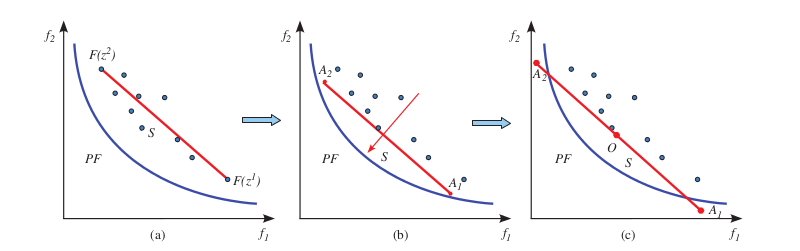
\includegraphics[width=0.7\linewidth]{./img/approximate_pareto_optimal}
\caption{Approximate Pareto-optimal set}
\label{fig:approximate_pareto_optimal}
\end{figure}


\section{Stepwise uncertainty reduction}

\begin{itemize}
\item [\textbf{2013}] Multiobjective optimization using Gaussian process emulators via
stepwise uncertainty reduction~\cite{picheny2013multiobjective}
\item [\textbf{2014}] A stepwise uncertainty reduction approach to constrained global optimization~\cite{picheny2014stepwise}
\end{itemize}

\emph{Stepwise uncertainty reduction} (SUR strategy) is used to reduce an uncertainty measure by sequential sampling about a quantity of interest.
The objective space is decomposed into cells, which are hyper-rectangles $ \Omega_{i} $.
A set of non-dominated cells $ I^{*} $ can be found by comparing with all other cells.

\emph{Improvement} is defined as the difference between the current observed minimum and the new function value if it is positive, or zero otherwise, which is written as $ \max(0, u^{min}_{n}-Y(x)) , y^{min}_{n} = \min(y_{1}, \cdots , y_{n}) $.
\emph{Expected improvement} is conditional expectation under the GP model
$ EI(x) = E[ \max(0, u^{min}_{n}-Y(x)) \mid A_{n} ] $.
The new measurement is selected as $ x_{n+1} = \arg \max_{x \in X} EI(x) $.

\section{Singular Continuation}

\begin{itemize}
\item [\textbf{2011}] Singular Continuation: Generating Piecewise Linear Approximations to Pareto Sets via Global Analysis~\cite{doi:10.1137/100784746}
\end{itemize}

Sometimes the global representation of the Pareto set is not always non-convex.

Pareto critical set

\bibliographystyle{spiebib}
\bibliography{reference}

\end{document}